\documentclass[ignorenonframetext,]{beamer}
\setbeamertemplate{caption}[numbered]
\setbeamertemplate{caption label separator}{: }
\setbeamercolor{caption name}{fg=normal text.fg}
\beamertemplatenavigationsymbolsempty
\usepackage{lmodern}
\usepackage{amssymb,amsmath}
\usepackage{ifxetex,ifluatex}
\usepackage{fixltx2e} % provides \textsubscript
\ifnum 0\ifxetex 1\fi\ifluatex 1\fi=0 % if pdftex
  \usepackage[T1]{fontenc}
  \usepackage[utf8]{inputenc}
\else % if luatex or xelatex
  \ifxetex
    \usepackage{mathspec}
  \else
    \usepackage{fontspec}
  \fi
  \defaultfontfeatures{Ligatures=TeX,Scale=MatchLowercase}
\fi
% use upquote if available, for straight quotes in verbatim environments
\IfFileExists{upquote.sty}{\usepackage{upquote}}{}
% use microtype if available
\IfFileExists{microtype.sty}{%
\usepackage{microtype}
\UseMicrotypeSet[protrusion]{basicmath} % disable protrusion for tt fonts
}{}
\newif\ifbibliography
\hypersetup{
            pdftitle={Project 10 - Missing values and LASSO},
            pdfauthor={Erik Bülow, Markus Ingvarsson, Debbie Lau},
            pdfborder={0 0 0},
            breaklinks=true}
\urlstyle{same}  % don't use monospace font for urls

% Prevent slide breaks in the middle of a paragraph:
\widowpenalties 1 10000
\raggedbottom

\AtBeginPart{
  \let\insertpartnumber\relax
  \let\partname\relax
  \frame{\partpage}
}
\AtBeginSection{
  \ifbibliography
  \else
    \let\insertsectionnumber\relax
    \let\sectionname\relax
    \frame{\sectionpage}
  \fi
}
\AtBeginSubsection{
  \let\insertsubsectionnumber\relax
  \let\subsectionname\relax
  \frame{\subsectionpage}
}

\setlength{\parindent}{0pt}
\setlength{\parskip}{6pt plus 2pt minus 1pt}
\setlength{\emergencystretch}{3em}  % prevent overfull lines
\providecommand{\tightlist}{%
  \setlength{\itemsep}{0pt}\setlength{\parskip}{0pt}}
\setcounter{secnumdepth}{0}

\title{Project 10 - Missing values and LASSO}
\author{Erik Bülow, Markus Ingvarsson, Debbie Lau}
\date{updated: 2019-05-12}

\begin{document}
\frame{\titlepage}

\begin{frame}{Methodology}

\begin{block}{Simulate data}

\begin{itemize}
\tightlist
\item
  n = 1000
\item
  p = 50
\item
  0 \(\leq\) proportion of unrelated features \(\leq\) 1
\item
  random from standard normal, exponential and uniform distributions
\item
  0 \(\leq\) proportion of missing values \textless{} 1
\item
  Missing Completely at Random (MCAR)
\end{itemize}

\end{block}

\end{frame}

\begin{frame}{Methodology}

\begin{block}{Imputation}

\begin{itemize}
\tightlist
\item
  mean
\item
  median
\item
  bagging
\item
  KNN
\end{itemize}

\end{block}

\end{frame}

\begin{frame}{Goals}

\begin{block}{1. Sensitivity of LASSO with missing values}

\end{block}

\begin{block}{2. Compare LASSO and Dantzig Selector}

\end{block}

\end{frame}

\begin{frame}{LASSO and Dantzig Selector}

\begin{itemize}
\item
  Methods for feature selection by penalized regression
\item
  Family of LASSO {[}1{]}
\end{itemize}

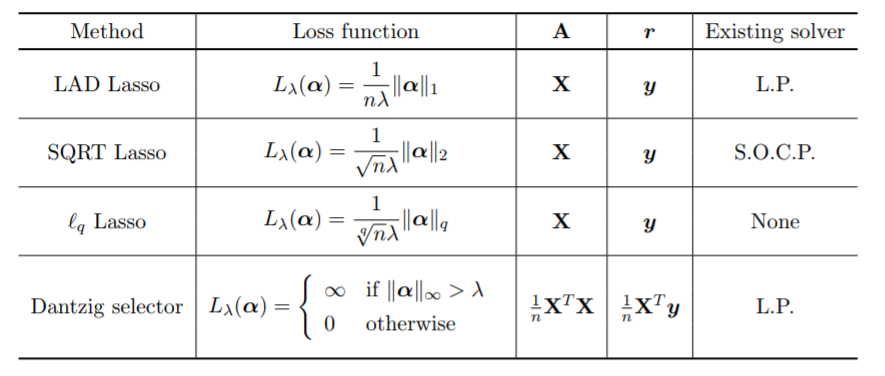
\includegraphics[width=0.8\linewidth]{dantzig_table}

\end{frame}

\begin{frame}{Result 1: Sensitivity of LASSO with missing values}

\end{frame}

\begin{frame}{}

\end{frame}

\begin{frame}{}

\end{frame}

\begin{frame}{}

\end{frame}

\begin{frame}{Result 2: Compare LASSO and Dantzig Selector}

\begin{itemize}
\tightlist
\item
  Proportion of missing data: 30\%
\item
  Without unrelated features
\end{itemize}

\end{frame}

\begin{frame}{}

\end{frame}

\begin{frame}{Summary}

\begin{block}{Result 1}

\begin{itemize}
\tightlist
\item
  The higher proportion of missing data the worse performance of LASSO
\end{itemize}

\end{block}

\begin{block}{Result 2}

\begin{itemize}
\tightlist
\item
  Do not show big difference between two models
\item
  Absolute values of coefficients bigger for Dantzig Selector
\end{itemize}

\end{block}

\begin{block}{Future work}

\begin{itemize}
\tightlist
\item
  Compare LASSO and Dantzig Selector under different proportions of
  unrelated features
\end{itemize}

\end{block}

\end{frame}

\begin{frame}{Reference}

{[}1{]} X. Li, T. Zhao, X. Yuan, and H. Liu. An R package flare for high
dimensional linear regression and precision matrix estimation.
\url{http://cran.r-project.org/web/packages/flare}, 2015.

\end{frame}

\end{document}
